\section{Related works}
\subsection{Leetcode}

\begin{figure}[h!]
    \centering
    
\includegraphics[width=1\textwidth]{Contents/Chapter 1/Images/Leetcode.png}
    \vspace{0.6cm}
    \caption{Leetcode Homepage}
    \label{fig:leetcode-system}
\end{figure}

LeetCode, founded in 2015 based on the co-founders’ experiences working at Google and Amazon, has become a highly popular online coding platform that offers a large collection of programming problems for all skill levels. It offers a comprehensive environment where users can practice a wide variety of programming problems, engage with a global community, and track their progress over time.LeetCode is widely recognized for its role in fostering problem-solving abilities and strengthening algorithmic thinking, making it an essential tool for both students and professionals in the software engineering field.\\

Key features of LeetCode include:
\begin{itemize}
    \item \textbf{Extensive Problem Library:} Thousands of coding problems across multiple difficulty levels and topics.
    \item \textbf{Online Code Editor:} Supports multiple programming languages with instant feedback and test case evaluation.
    \item \textbf{Contest and Challenge System:} Regular coding contests to benchmark skills against a global community.
    \item \textbf{Interview Preparation Kits:} Curated problem sets designed to prepare users for technical interviews at top tech companies.
    \item \textbf{Discussion Forums:} Active community discussions for problem-solving strategies, solutions, and learning resources.
    \item \textbf{Progress Tracking and Analytics:} Tools to monitor performance, problem-solving patterns, and skill improvement over time.
\end{itemize}

LeetCode offers a diverse set of core features that comprehensively address the needs of different user roles, including problem solving, submission tracking, contest participation, community interaction, ranking, and interview preparation. These features collectively enhance the learning experience, promote skill development, and encourage active engagement within the platform. However, it is noteworthy that LeetCode currently does not provide a public leaderboard to foster a stronger competitive environment among users.
\subsection{Codeforces}

\begin{figure}[h!]
    \centering
    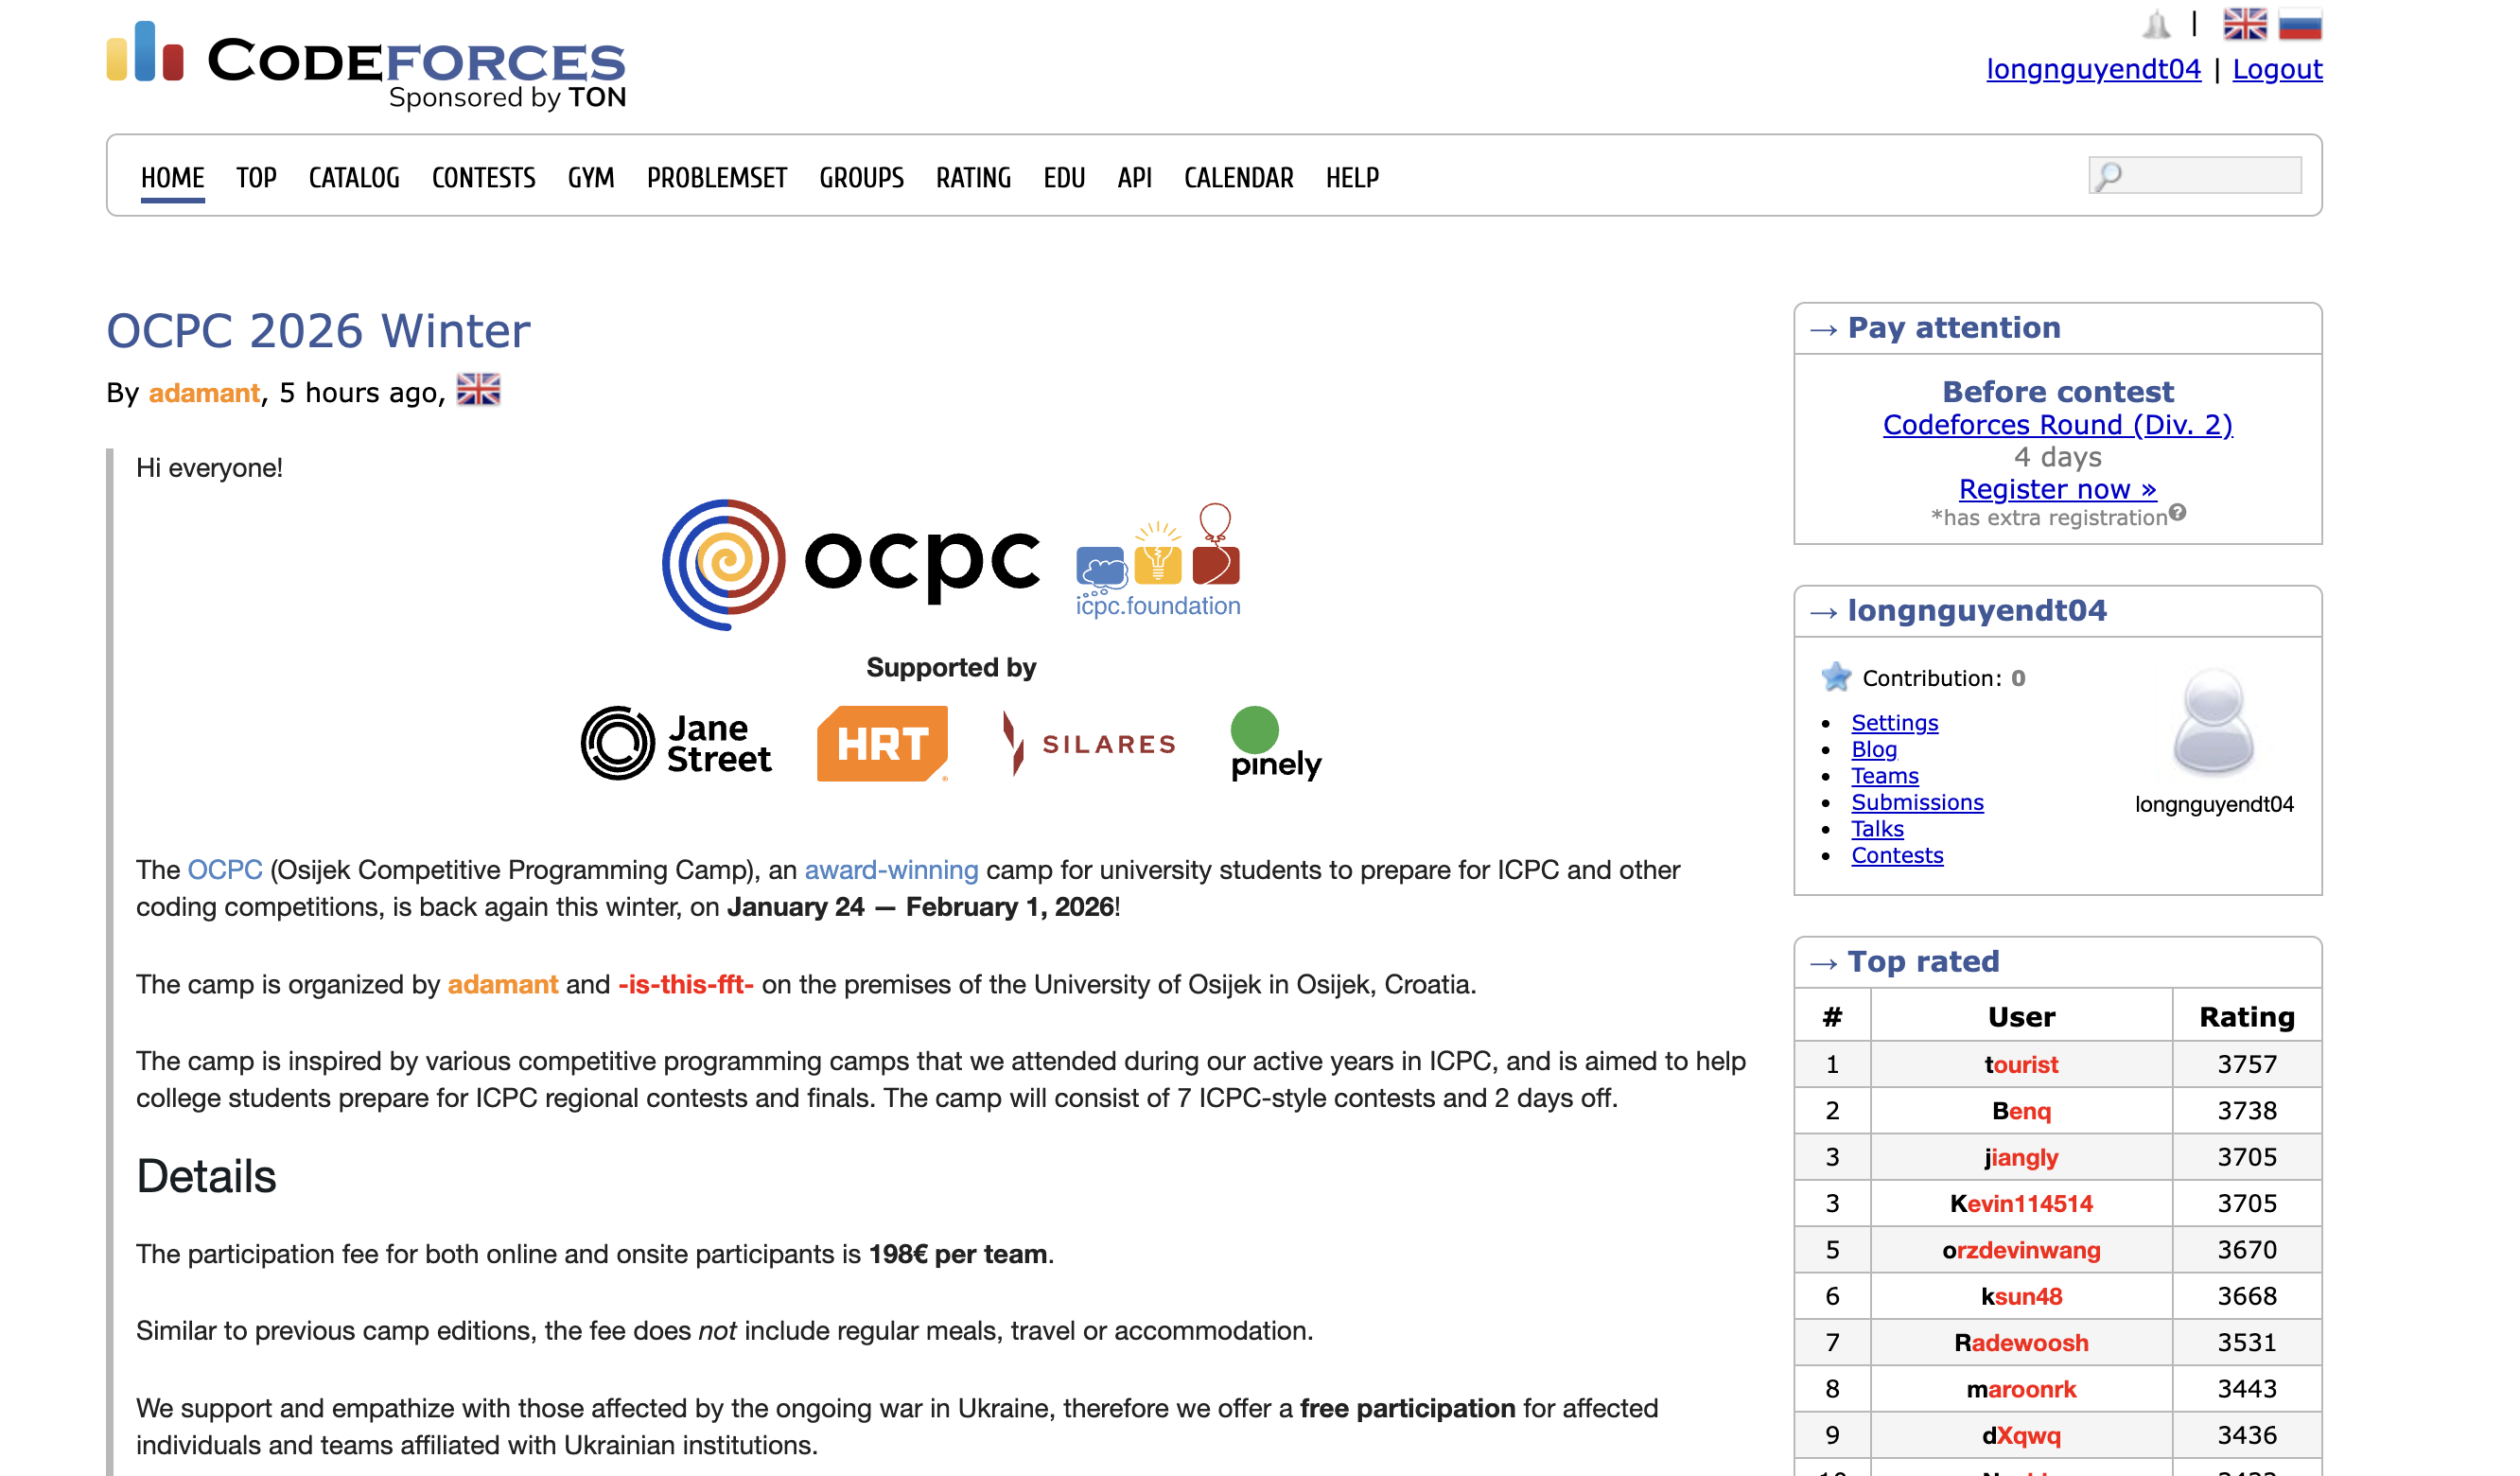
\includegraphics[width=1\textwidth]{Contents/Chapter 1/Images/Codeforces.png}
    \vspace{0.6cm}
    \caption{Codeforces Homepage}
    \label{fig:codeforces-system}
\end{figure}

Codeforces is a prominent online platform dedicated to competitive programming, offering users a structured environment to enhance their algorithmic and problem-solving skills through real-time contests. It is widely used by students, professionals, and competitive programmers to benchmark their abilities and engage with a global community of coders.\\

Key features of Codeforces include:
\begin{itemize}
    \item \textbf{Extensive Problem Sets:} A vast collection of algorithmic and programming problems across multiple difficulty levels.
    \item \textbf{Online Contests:} Regular timed competitions, including rated contests, that simulate real-world competitive programming scenarios.
    \item \textbf{Integrated Code Editor:} Supports multiple programming languages with submission, testing, and evaluation against problem test cases.
    \item \textbf{Community Discussion:} Active forums for problem discussions, solution sharing, and peer feedback.
    \item \textbf{User Ratings and Rankings:} Automatic rating system reflecting performance in contests and overall ranking among users globally.
    \item \textbf{Problem Tags and Difficulty Filters:} Tools to browse and search problems efficiently based on difficulty, topic, and tags.
\end{itemize}

Codeforces excels in providing a practical, competition-oriented environment that strengthens real-world programming and algorithmic skills. Its focus on timed contests and rigorous problem solving makes it an excellent platform for users aiming to improve performance in competitive programming. However, Codeforces does not currently provide dedicated tools for technical interview preparation, such as virtual assistants, hints, or structured interview question sets.

\subsection{VNOI Online Judge}

\begin{figure}[h!]
    \centering
    
\includegraphics[width=1\textwidth]{Contents/Chapter 1/Images/VNOI.png}
    \vspace{0.6cm}
    \caption{VNOI Online Judge Homepage}
    \label{fig:vnoi-system}
\end{figure}

VNOI Online Judge (VNOJ) is the official online judge system of the Vietnam Olympiad in Informatics community. The platform is based on the open-source DMOJ system and was built to provide a dedicated environment for Vietnamese learners to practice programming, compete in contests, and access problem sets from national and international competitions. VNOJ also continues the role of the former VOJ system by preserving and expanding a large archive of Vietnamese competitive programming problems.\\

Key features of VNOI Online Judge include:
\begin{itemize}
    \item \textbf{Vietnamese Problem Archive:} A large collection of problems from Vietnamese contests, national excellent student exams, ACM-ICPC style contests, and VNOI official events.
    \item \textbf{Automatic Online Judge:} Submission evaluation with verdicts, execution limits, and support for competitive programming workflows.
    \item \textbf{Contest System:} Official and practice contests organized for the Vietnamese competitive programming community.
    \item \textbf{User Ranking:} Public user profiles and ranking information that encourage competition and long-term practice.
    \item \textbf{Community Knowledge Base:} Links to VNOI Wiki, blogs, news, and learning resources focused on algorithms and programming contests.
    \item \textbf{Vietnamese Community Focus:} Content, announcements, and educational activities are tailored to Vietnamese students and competitive programmers.
\end{itemize}

VNOI Online Judge is especially valuable for Vietnamese IT students because it provides localized content, familiar contest formats, and access to problem sets from domestic competitions. Its strengths are closely aligned with competitive programming education and community development in Vietnam. However, VNOJ focuses mainly on algorithm practice and contest participation, while CodeRank aims to combine these competitive features with broader learning support such as interview preparation, centralized real-time discussions, and customizable user-created contests.

\subsection{ Websites comparison}
\begin{table}[h!]
\centering
\renewcommand{\arraystretch}{1.3}
\caption{Comparison of existing website with CodeRank}
\label{tab:website-comparison}
\begin{tabularx}{\textwidth}{|l|X|X|X|X|}
\hline
\textbf{Criteria} & \textbf{LeetCode} & \textbf{Codeforces} & \textbf{VNOI Online Judge} & \textbf{CodeRank} \\
\hline
Problem Library & Yes & Yes & Yes & Yes \\
\hline
Online Coding Editor & Yes & Yes & Yes & Yes \\
\hline
Community & Active discussion forums & Active forums with contest discussions & Vietnamese competitive programming community, blogs, wiki, and announcements & Centralized real-time discussion forums \\
\hline
Contest System & Regular contests organized by platform & Timed contests with system-created schedule & Official and practice contests for the VNOI community & Both official and user-created contests, customizable by users. \\
\hline
Interview Preparation & Yes & No & No & Yes \\
\hline
Ranking System & Points for solved problems, but not visible to all users & Rating system based on contest performance & Public user rankings and contest standings & Dynamic points for problem solving and public centralized leaderboard \\
\hline
Multilingual & Support English \& Chinese & Support English \& Russian & Mainly Vietnamese with some English problem content & Support English \& Vietnamese \\
\hline
\end{tabularx}
\end{table}

\FloatBarrier

Obviously, each platform has its own strengths: LeetCode offers an extensive problem library and dedicated interview preparation resources, Codeforces emphasizes timed contests, rating systems, and community-driven forums for competitive practice, and VNOI Online Judge provides localized Vietnamese problem sets, contests, and learning resources for the national competitive programming community. However, CodeRank combines these advantages and adds key enhancements, including both official and user-created contests with customizable settings, a centralized public leaderboard, real-time discussion forums, and multilingual support (including Vietnamese). These features make CodeRank a comprehensive, user-centered platform tailored to the educational and practical needs of Vietnamese IT students.
